\documentclass{beamer}
\usepackage{geometry}
\usepackage[english]{babel}
\usepackage[utf8]{inputenc}
\usepackage{amsmath}
\usepackage{amsfonts}
\usepackage{amssymb}
\usepackage{tikz}
\usetikzlibrary{quotes, angles}
\usepackage{graphicx}
\usepackage{multicol}

%\usepackage{pgfplots}
%\pgfplotsset{width=10cm,compat=1.9}
%\usepackage{pgfplotstable}

\setlength{\headheight}{26pt}%doesn't seem to fix warning

\usepackage{fancyhdr}
\pagestyle{fancy}
\fancyhf{}

%\rhead{\small{3 September 2019}}
\lhead{\small{BECA / Dr. Huson / Geometry Unit 1}}

\renewcommand{\headrulewidth}{0pt}

\title{Mathematics Class Slides}
\subtitle{Bronx Early College Academy}
\author{Christopher J. Huson PhD}
\date{7-15 October 2020}

\begin{document}
\frame{\titlepage}
\section[Outline]{}
\frame{\tableofcontents}

\section{1.11 Review vocabulary and segment calculations, 14 October}
  \frame
  {
    \frametitle{GQ: How do we measure line segments?}
    \framesubtitle{CCSS: HSG.CO.A.1 Know precise geometric definitions  \hfill \alert{1.9 Wednesday 9 Oct}}
  
    \begin{block}{Do Now: Assignments self-assessment}
    \begin{enumerate}
        \item Check all assignments, they must be turned in today
        \item Have you completed Deltamath? Khan Academy? the 1.5 worksheet?
    \end{enumerate}
    \end{block}
    Lesson: 1.5 worksheet\\
    Construction of a perpendicular bisector \\
    Review and practice of vocabulary, line segments, and congruence
  }

  \frame
  {
    \frametitle{1) Diagrams and notation}
    Given the points $R$ and $S$, draw ray $\overrightarrow{SR}$.\\
    \vspace{2cm}
    \begin{center}
      \begin{tikzpicture}
      \draw [fill] (2,-1) circle [radius=0.05] node[below]{$R$};
      \draw [fill] (5,0) circle [radius=0.05] node[below]{$S$};
    \end{tikzpicture}
    \end{center} \vspace{1cm}
  }


  \frame
  {
    \frametitle{2) Diagrams and notation}
      In circle $O$, which radius is longer? $\overline{OB}$ or $\overline{OC}$
      \begin{enumerate}
        \item $OB > OC$
        \item $OB < OC$
        \item $OB = OC$
        \end{enumerate}
        \begin{tikzpicture}
          \draw [-, thick] (0,0)--(2,0) node [right]{$B$};
          \draw [-, thick] (0,0)--(135:2);
          \draw [thick] (0,0) circle [radius=2.0];
          \draw [fill] (0,0) circle [radius=0.05] node[below]{$O$};
          \draw [fill] (2,0) circle [radius=0.05] node[right]{$B$};
          \draw [fill] (135:2) circle [radius=0.05] node[above left]{$C$};
          %\node at (1,0) [below]{$r = 2$};
        \end{tikzpicture}
  }

  \frame
  {
    \frametitle{3)  Diagrams and notation}
      Given isosceles $\triangle PQR$ with $\overline{PQ} \cong \overline{QR}$.\\[0.5cm]
      On the diagram mark the congruent line segments with tick marks. \vspace{1cm}
      \begin{center}
      \begin{tikzpicture}[scale=0.3]
        \draw [thick](0,0)--(9,0)--(4,8)--(0,0);
        \draw [fill] (0,0) circle [radius=0.05] node[below]{$P$};
        \draw [fill] (9,0) circle [radius=0.05] node[below]{$Q$};
        \draw [fill] (4,8) circle [radius=0.05] node[above right]{$R$};
      \end{tikzpicture}
      \end{center}
  }

  \frame
  {
    \frametitle{4)  Applying the segment addition postulate}
      Given $\overline{TUV}$, $TU=8.6$, and $TV=20.2$. Find ${UV}$.\\[0.5cm]
      Show your work by marking the diagram and writing an equation.\\[2cm]
        \begin{tikzpicture}
          \draw [-, thick] (0,0)--(7,0);
          \draw [fill] (0,0) circle [radius=0.05] node[below]{$T$};
          \draw [fill] (3,0) circle [radius=0.05] node[below]{$U$};
          \draw [fill] (7,0) circle [radius=0.05] node[below]{$V$};
        \end{tikzpicture} \vspace{4cm}
  }

  \frame
  {
    \frametitle{5) Applying the segment addition postulate}
      Find the perimeter of the isosceles $\triangle ABC$, given $\overline{AC} \cong \overline{BC}$, $AB=11$, and $AC=14 \frac{1}{2}$\\[0.5cm]
      Show your work with an equation for full credit.\\
        \begin{tikzpicture}[scale=0.5]
          \draw [thick](0,0)--(4,0)--(2,6)--(0,0);
          \draw [fill] (0,0) circle [radius=0.05] node[below]{$A$};
          \draw [fill] (4,0) circle [radius=0.05] node[below]{$B$};
          \draw [fill] (2,6) circle [radius=0.05] node[above right]{$C$};
          \draw [thick] (0.8,3)--(1.2,3); %tick mark
          \draw [thick] (2.8,3)--(3.2,3); %tick mark
          \node at (2,0) [below]{11};
          \node at (1,3.2) [left]{$14 \frac{1}{2}$};
        \end{tikzpicture}
  }

  \frame
  {
    \frametitle{6) Applying the segment addition postulate}
    Given $\overline{LMN}$, $LM=5x+3$, $MN=30$, $LN=43$. Find ${x}$.
    \begin{center}
       \begin{tikzpicture}
        \draw [-, thick] (0,0)--(7,0);
        \draw [fill] (0,0) circle [radius=0.05] node[below]{$L$};
        \draw [fill] (2,0) circle [radius=0.05] node[below]{$M$};
        \draw [fill] (7,0) circle [radius=0.05] node[below]{$N$};
        \node at (1,0) [above]{$5x+3$};
        \node at (4.5,0) [above]{$30$};
        \draw [<->, dashed] (0,-0.7)--(7,-0.7);
        \node at (3.5,-0.7) [below]{$43$};
      \end{tikzpicture}
    \end{center}
  \begin{enumerate}
      \item Write down an equation to represent the situation. \vspace{0.5cm}
      \item Solve for $x$. \vspace{2cm}
      \item Check your answer. \vspace{2cm}
    \end{enumerate}
  }

  \frame
  {
    \frametitle{7) Applying the segment addition postulate}
      Given equilateral $\triangle ABC$ having perimeter of 40. Find the length of side $\overline{AB}$, $x$. \vspace{1cm}
      \begin{center}
      \begin{tikzpicture}[scale=0.3]
        \draw [thick](0,0)--(9,0)--(4,8)--(0,0);
        \draw [fill] (0,0) circle [radius=0.05] node[below]{$A$};
        \draw [fill] (9,0) circle [radius=0.05] node[below]{$B$};
        \draw [fill] (4,8) circle [radius=0.05] node[above right]{$C$};
        \node at (4.5,0) [below]{$x$};
      \end{tikzpicture}
      \end{center}
  }

  \frame
  {
    \frametitle{8) Finding lengths on the number line}
    Given $G(-1)$ and $H(4)$, as shown on the number line. \\[0.25cm]
    Find the length of the line segment $\overline{GH}$.\\
      \begin{tikzpicture}
        \draw [<->] (-4.5,0)--(4.5,0);
        \draw [-, thick] (-1,0)--(4,0);
        \foreach \x in {-4,...,4} %2 leading for diff!=1
          \draw[shift={(\x,0)},color=black] (0pt,-3pt) -- (0pt,3pt) node[below=5pt]  {$\x$};
          \draw [fill] (-1,0) circle [radius=0.05] node[above] {$G$};
          \draw [fill] (4,0) circle [radius=0.05] node[above] {$H$};
      \end{tikzpicture} \\
      State an equation and the solution. \\[0.5cm]
  Check your work by counting the distance. Leave marks to show your work. \vspace{4cm}  
  }

  \frame
  {
    \frametitle{9) Finding lengths on the number line (spicy)}
    Given $S(1)$ and $T(3)$, as shown on the number line. \\[0.25cm]
    Find point $U$ given that point $T$ bisects $\overline{SU}$. Plot and label $U$ on the number line.\\[0.5cm]
      \begin{tikzpicture}
        \draw [<->] (-1.5,0)--(7.5,0);
        \draw [-, thick] (1,0)--(3,0);
        \foreach \x in {-1,...,7} %2 leading for diff!=1
          \draw[shift={(\x,0)},color=black] (0pt,-3pt) -- (0pt,3pt) node[below=5pt]  {$\x$};
          \draw [fill] (1,0) circle [radius=0.05] node[above] {$S$};
          \draw [fill] (3,0) circle [radius=0.05] node[above] {$T$};
      \end{tikzpicture} \vspace{4cm}  
  }

  \frame
  {
    \frametitle{10) Applying the segment addition postulate}
    Given $M$ is the midpoint of $\overline{AB}$, $AM=2x+5$, $MB=13$.
    \begin{enumerate}
      \item Mark the diagram with the values and tick marks
      \item Write an equation and solve for $x$
      \item Check your result
    \end{enumerate} \vspace{1cm}
      \begin{center}
        \begin{tikzpicture}
          \draw [fill] (0,0) circle [radius=0.05] node[below]{$A$};
          \draw [-, thick] (0,0)--(7,0);
          \draw [fill] (3.5,0) circle [radius=0.05] node[below]{$M$};
          \draw [fill] (7,0) circle [radius=0.05] node[below]{$B$};
          %\node at (1.7,0.5) [above]{$x+2$};
          %\node at (5.2,0.5) [above]{$11$};
          %\draw [<->, dashed] (0,-1)--(7,-1);
          %\node at (3.5,-1) [below]{$20$};
        \end{tikzpicture}
      \end{center} \vspace{4cm}
  }

  \frame
  {
    \frametitle{12) Applying the segment addition postulate}
      The points $Q$ and $R$ trisect the line segment $\overline{PS}$. $PS=13 \frac{1}{2}$.
      \begin{enumerate}
        \item Mark and label the approximate locations of $Q$ and $R$.
        \item Find ${PQ}$. State an equation for full credit.
      \end{enumerate} \vspace{1cm} 
      \begin{center}
        \begin{tikzpicture}
          \draw [-, thick] (0,0)--(7,0);
          \draw [fill] (0,0) circle [radius=0.05] node[below]{$P$};
          \draw [fill] (7,0) circle [radius=0.05] node[below]{$S$};
        \end{tikzpicture} 
      \end{center} \vspace{3cm} 
  }

\end{document}